% Propósito: enseñar qué magnitudes ocupan los ejes de una función
% desempeño--nivel y evitar que una curva aislada se interprete como lesión.
% Origen: descripción de la logoaudiometría de la sección
% \ref{sec:u8-logoaudiometria}. Curva cualitativa dibujada con Bézier; no
% procede de datos, no responde a una lista verbal y no es normativa.
% Descripción accesible: el eje horizontal representa el nivel de presentación
% en decibeles con la advertencia de que debe declararse la escala. El eje
% vertical representa respuestas correctas entre cero y cien por ciento.
% Puntos esquemáticos forman una curva creciente. Recuadros indican que cada
% punto depende del material, el procedimiento y la persona, y que la forma
% aislada no localiza una lesión.
% Validación prevista: comprobar que el eje horizontal no mezcla dB HL, dB SL
% y dB SPL, que el porcentaje se limita a 0--100 % y que no hay valores
% clínicos o normativos implícitos.
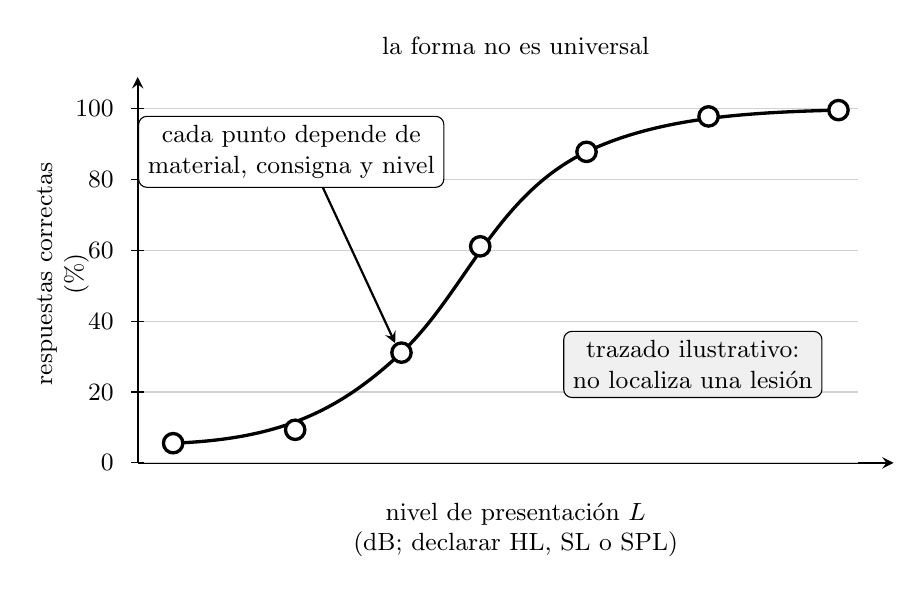
\begin{tikzpicture}[font=\small,>=stealth,x=1cm,y=1cm]
    \draw[->,thick] (1.20,0.80) -- (10.80,0.80);
    \draw[->,thick] (1.20,0.80) -- (1.20,5.70);
    \node[align=center] at (6.00,-0.05)
        {nivel de presentación \(L\)\\
         (\(\mathrm{dB}\); declarar HL, SL o SPL)};
    \node[rotate=90,align=center] at (0.25,3.20)
        {respuestas correctas\\(\(\%\))};

    \foreach \y/\lab in {0.80/0,1.70/20,2.60/40,3.50/60,4.40/80,5.30/100}{
        \draw[black!18] (1.20,\y) -- (10.35,\y);
        \draw (1.12,\y) -- (1.28,\y);
        \node[anchor=east] at (1.02,\y) {\lab};
    }

    \draw[very thick]
        (1.65,1.05)
        .. controls (3.00,1.10) and (3.75,1.45) .. (4.55,2.20)
        .. controls (5.35,2.95) and (5.75,4.20) .. (6.90,4.75)
        .. controls (7.80,5.18) and (8.90,5.25) .. (10.10,5.28);

    \foreach \x/\y in {
        1.65/1.05,3.20/1.22,4.55/2.20,5.55/3.55,
        6.90/4.75,8.45/5.20,10.10/5.28}{
        \fill[white] (\x,\y) circle (3.5pt);
        \draw[very thick] (\x,\y) circle (3.5pt);
    }

    \node[draw,rounded corners=3pt,fill=white,align=center]
        at (3.15,4.75)
        {cada punto depende de\\
         material, consigna y nivel};
    \draw[->,thick] (3.55,4.30) -- (4.47,2.32);

    \node[draw,rounded corners=3pt,fill=black!6,align=center]
        at (8.25,2.05)
        {trazado ilustrativo:\\
         no localiza una lesión};
    \node[align=center] at (6.00,6.10)
        {la forma no es universal};
\end{tikzpicture}
